\documentclass[a4, 12pt]{article}

\usepackage[utf8]{inputenc}
\usepackage[margin=1in]{geometry}
\usepackage{float}
\usepackage{caption}
\usepackage{subcaption}
\usepackage{multirow}
\usepackage{datetime}
\usepackage{pifont}
\usepackage[round, sort, numbers]{natbib}
\usepackage{cite}

\usepackage[toc,page]{appendix}
\usepackage{listings}
\usepackage{amsmath}

\usepackage[pdftex]{graphicx}
\usepackage{wrapfig}
\usepackage[hidelinks]{hyperref}
\usepackage{tabularx}

\usepackage{color, colortbl}
\usepackage{booktabs}

% More space between rows:
\renewcommand{\arraystretch}{1.1}

% Slightly more space between columns:
\setlength{\tabcolsep}{8pt}

% Headers & Footers
\usepackage{fancyhdr} % This should be set AFTER setting up the page geometry
\setlength{\headheight}{15.6pt}
\pagestyle{fancy} % options: empty , plain , fancy
\fancyhf{}
\renewcommand{\headrulewidth}{0.4pt} % customise the layout...
\lhead{\textsc{Radboud University Nijmegen}}\chead{}\rhead{\textsc{Burger, Kruijswijk, Strobel \& Wijnands}}
\lfoot{}\cfoot{\thepage}\rfoot{\textsc{}}
\newcommand{\HRule}{\rule{\linewidth}{0.5mm}}

\definecolor{Gray}{gray}{0.8}

% Tikz package includes
\usepackage{tikz}
\usetikzlibrary{shapes,arrows,automata,positioning}	

% Custom caption type
\DeclareCaptionType{capeq}[][List of equations]
\captionsetup[capeq]{name=Equation}
\captionsetup{font=scriptsize}

\lstset	{
	captionpos=b
}

% Define block styles
\tikzstyle{decision} = [diamond, draw, fill=blue!20, 
    text width=4.5em, text badly centered, node distance=3cm, inner sep=0pt]
\tikzstyle{block} = [rectangle, draw, fill=blue!20, 
    text width=5em, text centered, rounded corners, minimum height=4em]
\tikzstyle{line} = [draw, -latex']
\tikzstyle{cloud} = [draw, ellipse,fill=red!20, node distance=3cm,
    minimum height=2em]
    
%----------------------------------------------------------------------------------------
%	TITLE SECTION
%----------------------------------------------------------------------------------------

\newcommand{\horrule}[1]{\rule{\linewidth}{#1}} % Create horizontal rule command with 1 argument of height

%If we don't use a title page
%\title{
%\normalfont \normalsize 
%\textsc{Advanced Research Methods} \\ [25pt] % Your university, school and/or department name(s)
%\huge \textbf{Artificial Grammar Learning using Rapid Serial Visual Presentation} \\ % The article title
%}
%
%\author{F. Burger, J. Kruijswijk, V. Strobel, I. Wijnands} % Authors
%

\date{\normalsize\today} % Today's date or a custom date

\begin{document}
%If we use a title page
\begin{titlepage}
\begin{center}

\textsc{\LARGE Radboud University Nijmegen}\\[1cm]

% Upper part of the page. The '~' is needed because \\
% only works if a paragraph has started.

\includegraphics[width=0.15\textwidth]{media/ru-logo}~\\[1cm]

\textsc{\Large Advanced Research Methods}\\[0.6cm]

% Title
\HRule \\[0.4cm]
{ \huge \bfseries Artificial Grammar Learning using Rapid Serial Visual Presentation \\[0.4cm] }

\HRule \\[1.2cm]

% Author and supervisor
%\begin{minipage}{0.45\textwidth}
\begin{flushleft} \large
\emph{\textbf{Authors:}}\\
Franziska Burger (s4500466)\\
Jules Kruijswijk (s4140230)\\
Volker Strobel (s4491491)\\
Inez M. Wijnands (s4149696)\\
\emph{Radboud University Nijmegen}\\
\end{flushleft}
%\end{minipage}
\begin{flushleft} \large
%\begin{minipage}{0.4\textwidth}
\emph{\textbf{Supervisor:}} \\
Dr. Makiko Sadakata\\
\emph{Donders Institute for Brain,\\
Cognition and Behaviour}\\
%\vspace{0.35cm}
%Dr.~P.A. \textsc{Kamsteeg}\\
%Radboud University Nijmegen\\
%\end{minipage}
\end{flushleft}


\vfill

% Bottom of the page
SOW-MKI42a Advanced Research Methods\\
Artificial Intelligence\\
Faculty of Social Sciences\\
Radboud University Nijmegen\\
\vspace{0.2cm}
\date{\large\today} % Today's date or a custom date}

\end{center}
\end{titlepage}

\newpage
\pagenumbering{arabic}
\setcounter{page}{1}

%Abstract 
\begin{abstract}

\end{abstract}

%Introduction
\section{Introduction}
In our society today, a surefire way of making profit is by developing methods and tools that promise to help us manage life in the fast lane. One of the older methods with this purpose that is gaining in popularity again is the rapid intake of written information, also known as speed reading.
\subsection{Speed Reading} 
Interest in increasing one's reading rate was sparked when \citeauthor{javal1879essai} drew attention to eye movements during reading through a series of articles published in the 1870s \citep{javal1879essai, huey1908psychology, wade2009did}. Rather than reading words letter by letter, reading was now seen as an alternating process of fixations and saccades. Each fixation allows good readers to take in on average approximately three words. During saccades, nothing can be seen \citep{ahuja1995increase}. Research was fueled further after the American psychologist \citeauthor{renshaw1945visual} employed tachistoscopes to train pilots of the U.S. Navy in the second World War \citep{godnig2003tachi, benschop1998tachistoscope, renshaw1945visual}. A tachistoscope is an apparatus that allows the rapid serial visual presentation (RSVP) of stimuli. With this method, saccades could be eliminated by presenting words in the same location. 
%"Interest in the conditioning or control of eye movement resulted in the making of many other tachistoscopic devices such as the \textit{Reading Accelerator}, the \textit{Reading Rate Controller}, the \textit{Fashmeter}, and the \textit{Rate Reader}"\citep[p.~104]{witty1969rate}. 
The research regarding the effectiveness of RSVP to increase reading speed produced converging evidence that comprehension suffers under this approach \citep{swalm1973speed, witty1969rate, causey1954colleges, bormuth1961tachistoscope, mcconkie1973experimental, schotter2014don}. Despite such evidence, using RSVP for speed reading has recently resurfaced in popular culture in the form of smartphone and wearable applications, such as the one by Spritz \footnote{http://www.spritzinc.com/}. Several studies have shown the importance of reading in first and second language acquisition, with reading improving not only comprehension but also inducing an intuition of the underlying syntactic structure \citep{chomsky1972stages, siegel1988development,krashen1993power}. Thus, we are not quite ready to write off RSVP as a method for speed reading yet. In this project, we study the possibilities of the method in artificial grammar learning (AGL).

\subsection{Artificial Grammar Learning}
In the 1960s, \citeauthor{reber1967implicit} studied the implicit learning of stimulus structure. By conducting a series of experiments, he defined three requirements \citep[p.~190]{reber1978analogic} for such learning to occur:
\begin{enumerate}
\item The rules governing the stimulus material must be complex.
\item Participants should pay close attention to stimuli without searching for underlying rules.
\item Participants should be unable to verbalize the knowledge they obtained during learning. 
\end{enumerate}
\citeauthor{reber1967implicit} employed artificial grammars to ensure meeting the first requirement. Artificial grammars are finite state machines with the transition from one state to the next corresponding to one element of the grammar. Grammatical patterns, or words, are created by making only allowed transitions from the start state to the final state (see Figure\ref{figure1}). 
\begin{figure}
\centering
\hspace*{-1.55cm}
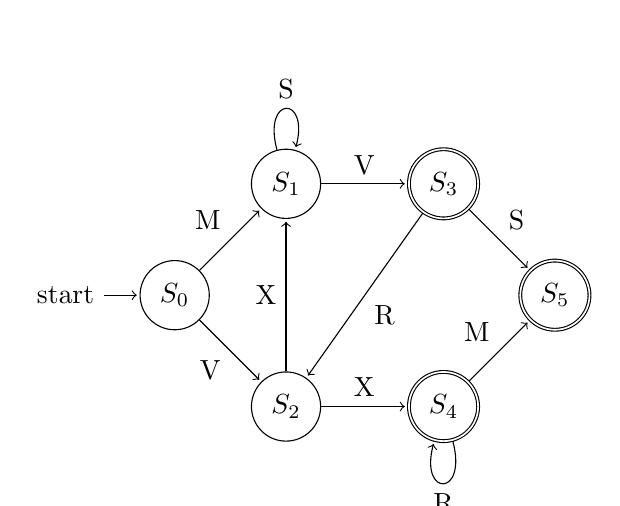
\begin{tikzpicture}[shorten >=1pt,node distance=2cm,on grid,auto] 
   \node[state,initial] (S_0)   {$S_0$}; 
   \node[state] (S_1) [above right=of S_0] {$S_1$}; 
   \node[state] (S_2) [below right=of S_0] {$S_2$}; 
   \node[state,accepting] (S_3) [right=of S_1] {$S_3$}; 
   \node[state,accepting] (S_4) [right=of S_2] {$S_4$}; 
   \node[state,accepting](S_5) [below right=of S_3] {$S_5$};
    \path[->] 
    (S_0) edge  node {M} (S_1)
          edge  node [swap] {V} (S_2)
    (S_1) edge  node  {V} (S_3)
          edge [loop above] node {S} ()
    (S_2) edge  node {X} (S_4)
          edge  node {X} (S_1)
    (S_3) edge  node  {R} (S_2)
          edge  node  {S} (S_5)
    (S_4) edge  node  {M} (S_5)
          edge [loop below] node {R} ();
\end{tikzpicture}
\caption{An artificial grammar is given by a finite state machine. States are indicated by circles labeled $S_{i}$. $S_{0}$ is the initial state. Every grammatical item has to start with a transition via an arrow from the initial state to a state directly connected to it (in this case $S_{1}$ or $S_{2}$). States encircled by two lines are final states ($S_{3}$, $S_{4}$, $S_{5}$). The machine can be exited from any final state. The arrows indicate legal transition directions (in this example, it is legal to move from $S_{3}$ to $S_{2}$ but not the other way around). Words are formed by concatenating the letters assigned to each arrow in the order of making the transition (grammatical words are for example MVS, VXRRR).} 
\label{figure1}
\end{figure}
%Insert some figure of an AG with a nice caption explaining how words are formed
The AGL paradigm consists of a learning and a testing phase. In the learning phase, participants are confronted with a set of grammatical words\footnote{In his initial studies \citep{reber1967implicit}, Reber asked participants to memorize these but later went on to study learning by mere exposure \citep{reber1978analogic}.}. In the testing phase, acquired knowledge is tested by presenting new words and asking participants to judge their grammaticality. 
This raises the question: How is it possible to develop a feeling for apparently nonsensical patterns? One theory is that implicit learning is statistical learning. This means that the grammatical patterns in the training phase are used to train a classifier within the brain, which tells us the probability for a new stimulus to be a word of the grammar or not \citep{perruchet2006implicit,saffran2002constraints}.
While \citeauthor{reber1967implicit} exposed participants to a total of 20 exemplars three times and each exemplar was regarded for ten seconds \citep{reber1978analogic}, later studies showed similar results for shorter exposure \citep{knowlton1996artificial,gomez1999artificial}\footnote{\citeauthor{knowlton1996artificial} exposed participants to stimuli for three seconds per item and then asked them to reproduce the item. When participants could not get it correct on this reproduction attempt, this could be repeated twice, so that theoretically participants could have seen items for a total of nine seconds. However, it is mentioned that few participants needed a third exposure to reproduce the item correctly. \citeauthor{gomez1999artificial} exposed 1 year-old toddlers to auditory exemplars of an artificial grammar that included vowels for a total of two minutes.}.\\
In this project, we are interested in the possibility of implicitly learning an artificial grammar by viewing exemplars presented in an RSVP paradigm. Specifically, we examine two research questions:
\begin{enumerate}
\item \label{item1}Does AGL occur when words are presented individually at the same location at a normal reading rate?
\item \label{item2}Does it also occur at faster presentation speeds (as used by speed reading tools) when
\begin{enumerate}
\item \label{item2a}the same amount of material is presented?
\item \label{item2b}material is presented for the same amount of time? 
\end{enumerate}
\end{enumerate}
To our knowledge, the limitations of AGL have not yet been studied with regard to the presentation speed of exemplars. We generally regard AGL as possible when exemplars are presented at normal and rapid speeds. This is due to the high attentional demand of RSVP (REFERENCE NEEDED) in combination with the importance of attention in implicit learning. However, if implicit learning is statistical learning, we further believe that longer exposure times will most likely lead to more reliable probabilistic inferences, with a repeated exposure potentially making up for a shorter exposure. Therefore, we expect an affirmative answer to research questions \ref{item1} and \ref{item2b}. 

 

%Methods
%\section{Methods}
\label{sec:method}

\subsection{Participants}
Ten right-handed healthy subjects participated in this experiment (three females, seven males; age: 19$-$26 years (mean = 20.9 years; S.E. = 2.1 years)). The experiment was approved by the ethical committee of the Faculty of Social Sciences of the Radboud University and all the participants gave informed consent.\\
\\
Participants were primarily found amongst AI students at the Radboud University. Participants were excluded from the experiment when they exhibit certain symptoms or disorders, amongst epilepsy and dyslexia. The following exclusion criteria were used:
\begin{itemize}
	\item Cognitive deficits that made comprehension of the information letter and intructions difficult, or motor impairment that made comprehension of the task or pushing a button impossible.
	\item Epilepsy. We used flickering stimuli in the experiment.
	\item Dyslexia. We used artificial words in the experiment and the participant should have no trouble distinguishing between letters and registering the order of letters.
\end{itemize}

\subsection{Experimental paradigm}
%procedure


%paradigm


%\begin{figure}[h]
%	\centering
%	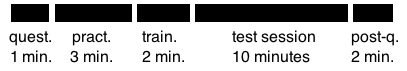
\includegraphics[width=\textwidth]{media/timeline-experiment}
%	\caption{Figure \ref{fig:timeline} shows the estimated timeline, not including breaks, of the experiment. The experiment starts with the BIT, capfitting, calibrating the eyetracker and a practice session. The second session 'before prism' starts immediately after. The third session 'after prism' starts with 15 minutes of prism adaptation and the first 20 trials, followed by two times 10 minutes of prism adaptation and 20 trials.}
%	\label{fig:timeline}
%\end{figure}

%task
\subsubsection{Task}
\label{sec:task}


%\begin{figure}[h]
%	\centering
%	\includegraphics[width=\textwidth]{media/screenshots}
%	\caption{The timeline of a single trial is shown. The baseline is the fixation cross. The cue for direction of attention is given and the stimuli commence. After the stimuli, the system asks the participant how many Xs he has counted at the attended side and feedback is shown immediately after.}
%	\label{fig:screenshots}
%\end{figure}

%feedback
\subsubsection{Feedback}
\label{sec:feedback}




\subsection{Eyetracker}


\subsection{Preprocessing}


\subsection{Statistical analysis}



%Results
\section{Results}
The total number of correct classifications on the 100 test items, $P_{C}$, was determined for each participant. To compare observed to chance level performance, the Wilcoxon signed-rank test was employed for the \textit{normal} and the \textit{fast-time} conditions, while a one-sample t-test could be used for the \textit{fast-amount} condition. \footnote{The Shapiro-Wilk test was used to check whether the small samples per condition were drawn from a normally distributed population \citep{yazici2007comparison}} The tests were performed one-tailed because only above chance level performance was of interest. As can be seen from the results of these tests, illustrated in Table X (insert Table), no group performed significantly above chance. Therefore, it would not be sensible to make any statistical between-group comparisons. However, although not significant, both the \textit{normal} and the \textit{fast-amount} groups show weak indications that learning may have occurred. Luckily, there are other measures that can provide additional information on this matter.
\begin{table}[h]
\centering
\begin{tabular}{l l l l }
\toprule
\textbf{Group} & \textbf{Chance Level Comparison} & \textbf{\textit{p}-value} \\
\midrule
  normal      & Wilcoxon Signed Rank test        & .068 \\
  fast-amount & One-sample \textit{t}-test       & .057 \\
  fast-time   & Wilcoxon Signed Rank test        & .237 \\      
\bottomrule
\end{tabular}
\caption{TODO}
\end{table}
The 100 test items consisted of 50 unique items which were all repeated once. Thus, participants could classify each unique item in one of four ways:
\begin{enumerate}
\item Correct-Correct (CC): classified correctly on both presentations
\item Correct-Erroneous (CE): classified correctly on the first presentation but incorrectly on the second
\item Erroneous-Correct (EC): classified incorrectly on the first presentation but correctly on the second
\item Erroneous-Erroneous (EE): misclassified on both presentations
\end{enumerate}
The sum of CC and EE denotes overall consistency. Importantly, ``when the status of the item is known, it is always classified correctly; when it is not known, a guess is made.'' \citep[p.~227]{reber1989implicit}. Using this simple model as a basis, \citeauthor{reber1989implicit} states that CE, EC, and EE should not be statistically distinguishable from each other, since they all reflect guesses. On the other hand, if EE is significantly greater than the average of CE and EC, it can be inferred that judgments were based on rules that are not representative of the grammar. Furthermore, if the participants actually implicitly learned a correct albeit partial representation of the grammar, CC should be significantly higher than each of the other three variables. Finally, if the difference between CE and EC or EC and CE is significant, it is indicative of forgetting or learning during the testing phase respectively (for an in-depth discussion see \citet{reber1989implicit}). For each group, Table XX shows the means for the four variables. Intuitively, the illustrated behavior of our participants seems representative of guessing behavior on all test items. Paired t-tests for the various combinations of these variables (all are distributed normally within each group) confirms this intuition. EC and CE do not show a significant difference. Thus, there is neither evidence for learning nor for forgetting during the testing phase. When comparing EE to the average of CE and EC, $t(9) \leq -4.216$ and $p < .01$ was obtained for all groups. Furthermore, CC was only significantly higher than EE in the \textit{normal} group ($t(9)=1.843$, $p=.049$) with the \textit{fast-amount} group showing a trend ($t(9)=1.758$, $p=.057$). Taken together, this implies that all participants based a considerable amount of their decisions on rules that were not part of the grammar. Only in the \textit{normal} group (and possibly in the \textit{fast-amount} group) were significantly more correct than incorrect rules applied. However, it must be noted that these differences are much smaller and thus much move vague than in the artificial grammar learning literature.
\begin{table}[h]
\centering
\begin{tabular}{lllllll}
\toprule
& \multicolumn{6}{c}{\textbf{Group}} \\
\cmidrule{2-7}
\textbf{Parameter} & \multicolumn{2}{l}{\textbf{normal}} & \multicolumn{2}{l}{\textbf{fast-amount}} & \multicolumn{2}{l}{\textbf{fast-time}} \\
\midrule
 	    & Mean                       & SD                              & Mean & SD  & Mean & SD \\
\cmidrule(lr{.75em}){2-3}\cmidrule(lr{.75em}){4-5}\cmidrule(lr{.75em}){6-7}
$P_{C}$      & 53.3                       & 5.8                             & 52.9 & 5.2 & 50.9 & 4.8 \\
CC	    & 37.6                       & 5.8                             & 41.6 & 5.7 & 35.4 & 7.4 \\
CE 	    & 16.2                       & 6.8                             & 12.4 & 4.1 & 14.8 & 2.4 \\
EC	    & 15.4                       & 3.9                             & 10.2 & 5.7 & 16.2 & 1.9 \\
EE	    & 30.8                       & 7.5                             & 35.8 & 7.7 & 33.6 & 8.2 \\
consistency & 68.4                       &                                 & 77.4 &     & 50.9 & \\
\bottomrule
\end{tabular}
\caption{TODO}
\end{table}
Lastly, we correlated the number of languages participants speak as well as their prior speed reading experience with their $P_C$-scores across groups. Slightly negative but non-significant correlations were obtained: $r=-.30$, $p=.11$ for the number of languages and $r=-.23$, $p=.22$ for the speed reading experience.

%Discussion
%\input{discussion}

%Conclusion & Outlook
%\input{conclusion}

\newpage


\bibliographystyle{abbrvnat}
\bibliography{bibliography}


%\input{appendix}

\end{document}